\chapter{Évaluation Expérimentale}
\label{cp:evaluation}

Afin de valider les performances de notre stratégie, nous avons utilisé un script \texttt{sh}, qui permet de lancer plusieurs parties et de récupérer les résultats.
Ce script nous renvoie, pour un niveau donnée et un nombre de parties donné, le pourcentage de victoire, et le nombre moyen de déplacements effectués par le runner.

\section{Niveau 0}

\subsection{Résultats}

\begin{table}[!htpb]
    \begin{tabularx}{\textwidth}{lXXX}
        \toprule
        Pourcentage de victoire & Moyenne de déplacements & Moyenne de bombes \\
        \midrule
        100\% & 87.0 & 0.0 \\
        \bottomrule
    \end{tabularx}
    \caption{Résultats pour le niveau 0 sur 1000 parties}
    \label{tab:res-niveau-0}
\end{table}

\subsection{Analyse des défaites}

Il n'y a pas de défaites pour le niveau 0 et le nombre moyen de déplacements est entier, car n'y a pas d'ennemi, le runner prend toujours le même chemin.

\section{Niveau 1}

\subsection{Résultats}

\begin{table}[!htpb]
    \begin{tabularx}{\textwidth}{lXXX}
        \toprule
        Pourcentage de victoire & Moyenne de déplacements & Moyenne de bombes \\
        \midrule
        100\% & 125.0 & 0.0 \\
        \bottomrule
    \end{tabularx}
    \caption{Résultats pour le niveau 1 sur 1000 parties}
    \label{tab:res-niveau-1}
\end{table}

\subsection{Analyse des défaites}

Il n'y a pas de défaites pour le niveau 1 et le nombre moyen de déplacements est entier.
Pourtant il y a un ennemi, mais le runner le contourne, et prend toujours le même chemin.
\newline
On remarque que la seule mécanique qui rend le jeu non déterministe est la position des ennemis lorsqu'ils réapparaissent.
Or, le solution que trouve notre stratégie contourne les ennemis, donc si elle réussi le niveau une fois, elle le réussira toujours.

\section{Niveau 2}

\subsection{Résultats}

\begin{table}[!htpb]
    \begin{tabularx}{\textwidth}{lXXX}
        \toprule
        Pourcentage de victoire & Moyenne de déplacements & Moyenne de bombes \\
        \midrule
        100\% & 174.0 & 0.0 \\
        \bottomrule
    \end{tabularx}
    \caption{Résultats pour le niveau 2 sur 1000 parties}
    \label{tab:res-niveau-2}
\end{table}

\subsection{Analyse des défaites}

Il n'y a pas de défaites pour le niveau 2, pour les mêmes raisons que pour le niveau 1.

\section{Niveau 3}

\subsection{Résultats}

\begin{table}[!htpb]
    \begin{tabularx}{\textwidth}{lXXX}
        \toprule
        Pourcentage de victoire & Moyenne de déplacements & Moyenne de bombes \\
        \midrule
        98.2\% & 161.7 & 2.7 \\
        \bottomrule
    \end{tabularx}
    \caption{Résultats pour le niveau 3 sur 10000 parties}
    \label{tab:res-niveau-3}
\end{table}

\subsection{Analyse des défaites}

A faire

\newpage

\section{Niveau 4}

\subsection{Résultats}

\begin{table}[!htpb]
    \begin{tabularx}{\textwidth}{lXXX}
        \toprule
        Pourcentage de victoire & Moyenne de déplacements & Moyenne de bombes \\
        \midrule
        96.9\% & 189.4 & 1.5 \\
        \bottomrule
    \end{tabularx}
    \caption{Résultats pour le niveau 4 sur 10000 parties}
    \label{tab:res-niveau-4}
\end{table}

\subsection{Analyse des défaites}

A faire

\section{Niveau supplémentaire}

Afin de tester notre stratégie sur un niveau plus difficile, nous avons créé un niveau supplémentaire.
Il reprend les mêmes plateformes que le niveau 3, mais avec des ennemis en plus.

\begin{figure}[!htpb]
    \centering
    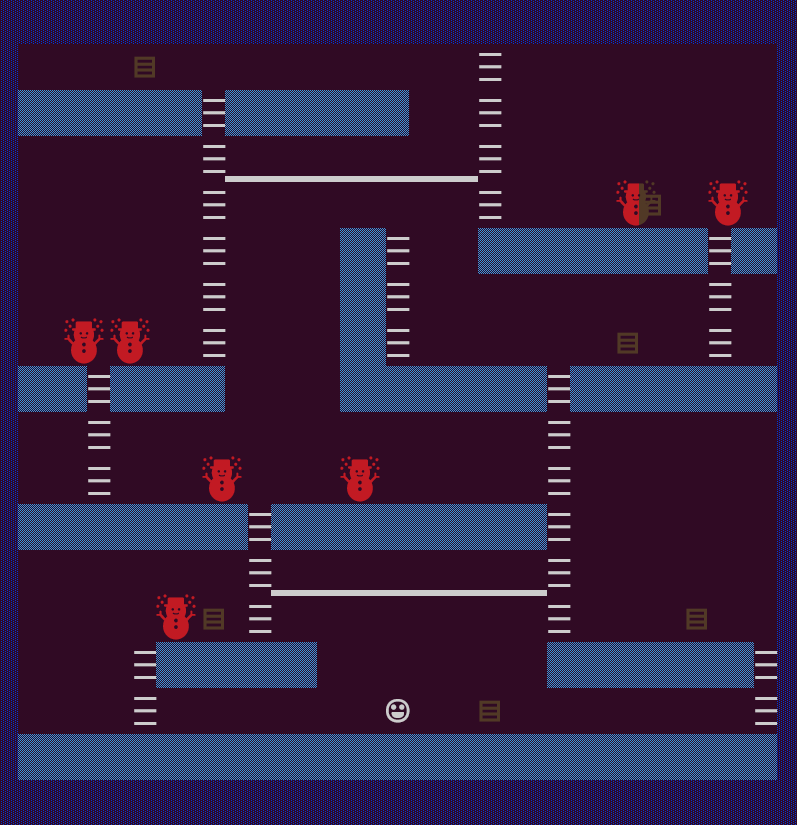
\includegraphics[width=0.5\textwidth]{Figures/level4.png}
    \caption{Niveau supplémentaire}
    \label{fig:niveau-supplementaire}
\end{figure}

\newpage

\subsection{Résultats}

\begin{table}[!htpb]
    \begin{tabularx}{\textwidth}{lXXX}
        \toprule
        Pourcentage de victoire & Moyenne de déplacements & Moyenne de bombes \\
        \midrule
        50.9\% & 209.2 & 13.9 \\
        \bottomrule
    \end{tabularx}
    \caption{Résultats pour le niveau supplémentaire sur 1000 parties}
    \label{tab:res-niveau-supplementaire}
\end{table}

\subsection{Analyse des défaites}

A faire